
\section{Introduction}
\label{sec:mdp-introduction}
This unit describes the very general formalism of Markov decision
processes (MDPs) for formalising problems in sequential decision
making.  Thus a \emindex{Markov decision process} can be used to model
stochastic path problems, stopping problems, reinforcement learning
problems, experiment design problems, and control problems.

We being by taking a look at the problem of \emindex{experimental
  design}. One instance of this problem occurs when considering how to
best allocate treatments with unknown efficacy to patients in an
adaptive manner, so that the best treatment is found, or so as to
maximise the number of patients that are treated successfully. The
problem, originally considered
by~\cite{Chernoff:SequentialDesignExperiments,chernoff1966smc},
informally can be stated as follows.

We have a number of treatments of unknown efficacy, i.e. some of them
work better than the others. We observe patients one at a time. When a
new patient arrives, we must choose which treatment to
administer. Afterwards, we observe whether the patient improves or
not. Given that the treatment effects are initially unknown, how can
we maximise the number of cured patients? Alternatively, how can we
discover the best treatment? The two different problems are formalised
below.

\begin{example}\indexmargin{Adaptive treatment allocation}
  Consider $k$ treatments to be administered to $T$ volunteers.  To each
  volunteer only a single treatment can be assigned.  At the $t$-th trial, we treat one volunteer with some treatment $a_t \in \{1, \ldots, k\}$. We then obtain  obtain a reward $r_t = 1$ if the patient is treated and $0$ otherwise.  We wish to choose actions maximising the utility  $U = \sum_t r_t$. This would correspond to maximising the number of patients that get treated over time.
\end{example}

\begin{example}\indexmargin{Adaptive hypothesis testing}
  An alternative goal would be to do a \emph{clinical trail}\index{clinical trial}, in order to find the best possible treatment. For simplicity, consider the problem of trying to find out whether a particular treatment is better or not than a placebo.  We are given a hypothesis set $\Omega$, with each $\omega \in \Omega$ corresponding to different models for the effect of the treatment and the placebo. Since we don't know what is the right model, we place a prior $\bel_0$ on $\Omega$. We can perform $T$ experiments, after which we must make decide whether or not the treatment is significantly better than the placebo. To model this, we define a decision set $\CD = \{d_0, d_1\}$ and a utility function $U : \CD \times \Omega \to \Reals$, which models the effect of each decision $d$ given different versions of reality $\omega$. One hypothesis $\omega \in \Omega$ is true. To distinguish them, we can choose
  from a set of $k$ possible experiments to be performed over $T$
  trials.  At the $t$-th trial, we choose experiment $a_t \in \{1,
  \ldots, k\}$ and observe outcome $x_t \in \CX$, with $x_t \sim
  P_\omega$ drawn from the true hypothesis. Our posterior is
  \[
  \bel_t(\omega) \defn
  \bel_0(\omega \mid a_1, \ldots, a_t, x_1, \ldots, x_t).
  \]
  The reward is $r_t = 0$ for $t < T$ and
  \[
  r_T = \max_{d \in D}\E_{\bel_T}(U \mid d).
  \]
  Our utility in this can again be expressed as a sum over individual rewards,  $U = \sum_{t=1}^T r_t$.
\end{example}
Both formalizations correspond to so-called {\em bandit problems} which we take a closer look at in the following section.

\section{Bandit problems}
\label{sec:exp-design-bandit}
\index{bandit problems}

The simplest bandit problem is the stochastic $n$-armed bandit.\index{bandit problems!stochastic} We are faced with $n$ different one-armed bandit machines, such as those found in casinos. In this problem, at time $t$, you have to choose one \emph{action} (i.e. a machine) $a_t \in \CA = \set{1, \ldots, n}$. In this setting, each time $t$ you play a machine, you receive a reward $r_t$, with fixed expected value $\omega_i = \E (r_t \mid a_t = i)$.
Unfortunately, you do not know $\omega_i$, and consequently the best arm is also unknown. How do you then choose arms so as to maximise the total expected reward? 
\begin{definition}[The stochastic $n$-armed bandit problem.]
  This is the problem of selecting a sequence of actions $a_t \in \CA$, with $\CA = \set{1, \ldots, n}$, so as to maximise expected utility, where the utility is 
  \[
  U = \sum_{t=0}^{T - 1} \disc^t r_t,
  \]
  where $T \in (0, \infty]$ is the horizon and $\gamma \in (0,1]$
  is a \emindex{discount factor}. The reward $r_t$ is stochastic,
  and only depends on the current action, with expectation $\E(r_t
  \mid a_t = i) = \omega_i$.
\end{definition}
In order to select the actions, we must specify some \emindex{policy} or decision rule. This can only depend on the sequence of previously taken actions and observed rewards. Usually, the policy $\pol :  \CA^* \times \Reals^* \to \CA$ is a deterministic mapping from the space of all sequences of actions and rewarsd to actions. That is, for every observation and action history $a_1, r_1, \ldots, a_{t-1}, r_{t-1}$ it suggests a single action $a_t$. However, it could also be a stochastic policy, that specifies a mapping to action distributions. We use the following notation for stochastic history-dependent bandit policies,
\begin{equation}
  \label{eq:history-dependent-bandit}
  \pol(a_t \mid a^{t-1}, r^{t-1})
\end{equation}
to mean the probability of actions $a_t$ given the history until time $t$.

How can we solve bandit problems? One idea is to apply the Bayesian
decision-theoretic framework we have developed earlier to maximise
utility in expectation.  More specifically, given the horizon $T
\in (0, \infty]$ and the discount factor $\disc \in (0,1]$, we
define our utility from time $t$ to be:
\begin{equation}
  \label{eq:reward-utility}
  U_t = \sum_{k=1}^{T-t} \gamma^k r_{t+k}.
\end{equation}
To apply the decision theoretic framework, we need to define a suitable family of probability measures $\family$, indexed by parameter $\omega \in \Omega$ describing the reward distribution of each bandit, together with a prior distribution $\bel$ on $\Omega$. Since $\omega$ is unknown, we cannot maximise the expected utility with respect to it. However, we can always maximise expected utility with respect to our belief $\bel$. That is, we replace the ill-defined problem of maximising utility in an unknown model with that of maximising expected utility given a distribution over possible models. The problem can be written in a simple form:
\begin{equation}
  \label{eq:bel-reward-utility}
  \max_\pol \E_\bel^\pol U_t = 
  \max_\pol \int_\Omega \E_\omega^\pol U_t \dd \bel{\omega}.
\end{equation}
The difficulty lies not in formalising the problem, but in the fact that the set of learning policies is quite large, rendering the optimisation infeasible.
The following figure summarises the statement of the bandit problem in the Bayesian setting.
\begin{block}{Decision-theoretic statement of the bandit problem}
  \begin{itemize}
  \item Let $\CA$ be the set of arms.
  \item Define a family of distributions $\family = \cset{P_{\omega, i}}{\omega \in \Omega, i \in \CA}$ on $\Reals$.
  \item Assume the i.i.d model $r_t \mid \omega, a_t = i \sim P_{\omega, i}$.
  \item Define prior $\bel$ on $\Omega$.
  \item Select a policy $\pol : \CA^* \times \Reals^* \to \CA$ maximising
    \[
    \E^\pol_\bel U = \E^\pol_\bel \sum_{t=0}^{T - 1} \disc^t r_{t}
    \]
  \end{itemize}
\end{block}
There are two main difficulties with this approach. The first is specifying the family and the prior distribution: this is effectively part of the problem formulation and can severely influence the solution. The second is calculating the policy that maximises expected utility given a prior and family. The first problem can be resolved by either specifying a subjective prior distribution, or by selecting a prior distribution that has good worst-case guarantees. The second problem is hard to solve, because in general, such policies are history dependent and the set of all possible histories is exponential in the horizon $T$.

\subsection{An example: Bernoulli bandits}
\label{sec:bernoulli-bandit-example}
As a simple illustration, consider the case when the reward for choosing one of the $n$ actions is either $0$ or $1$, with some fixed, yet unknown probability depending on the chosen action. This can be modelled in the standard Bayesian framework using the Beta-Bernoulli conjugate prior. More specifically, we can formalise the problem as follows.

Consider $n$ Bernoulli distributions with
unknown parameters $\omega_i$ ($i = 1, \ldots, n$) such that 
\begin{align}
  r_t \mid a_t = i &\sim
  \Bernoulli(\omega_i),
  &
  \E(r_t  \mid a_t = i) &= \omega_i.
\end{align}
Each Bernoulli distribution thus corresponds to the distribution of
rewards obtained from each bandit that we can play.  In order to
apply the statistical decision theoretic framework, we have to
quantify our uncertainty about the parameters $\omega$ in terms of a
probability distribution.

We model our belief for each bandit's
parameter $\omega_i$ as a Beta distribution $\BetaDist(\alpha_i,
\beta_i)$, with density $f(\omega \mid \alpha_i, \beta_i)$ so that
\[
\bel(\omega_1, \ldots, \omega_n)
=
\prod_{i=1}^n f(\omega_i \mid \alpha_i, \beta_i).
\]
Recall that the posterior of a Beta prior is also a Beta. Let
\[
N_{t,i} \defn \sum_{k=1}^t \ind{a_k = i}
\]
be the number of times we played arm $i$ and
\[
\hat{r}_{t,i} \defn \frac{1}{N_{t,i}} \sum_{k=1}^t r_t \ind{a_k = i}
\]
be the
\alert{empirical reward} of arm $i$ at time $t$. We
can let this equal $0$ when $N_{t,i} = 0$.
Then, the posterior distribution for the parameter of arm $i$ is
\[
\bel_t = \BetaDist(\alpha_i + N_{t,i} \hat{r}_{t,i}~,~ \beta_i + N_{t,i} (1 - \hat{r}_{t,i})).
\]
Since $r_t \in \{0,1\}$ the possible states of our belief given some
prior are $\Naturals^{2n}$.

In order for us to be able to evaluate a policy, we need to be able to
predict the expected utility we obtain. This only depends on our
current belief, and the state of our belief corresponds to the state
of the bandit problem.\indexmargin{belief state} This means that
everything we know about the problem at time $t$ can be summarised by
$\bel_t$. For Bernoulli bandits, sufficient statistic for our belief
is the number of times we played each bandit and the total reward from
each bandit.  Thus, our state at time $t$ is entirely described by our
priors $\alpha, \beta$ (the initial state) and the vectors
\begin{align}
  N_t = (N_{t,1}, \ldots, N_{t,i})\\
  \hat{r}_t = (\hat{r}_{t,1}, \ldots, \hat{r}_{t,i}).
\end{align}
At any time $t$, we can calculate the probability of observing
$r_t = 1$ or $r_t = 0$ if we pull arm $i$ as:
\[
\bel_t(r_t = 1 \mid a_t = i) = \frac{\alpha_i + N_{t,i} \hat{r}_{t,i}}{\alpha_i + \beta_i + N_{t,i}}
\]
So, not only we can predict the immediate reward based on our current
belief, but we can also predict all next possible beliefs: the next
state is well-defined and depends only on the current state.  As we
shall see later, this type of decision problem is more generally called a Markov
decision process (Definition~\ref{def:MDP}). For now, we shall more generally (and precisely) define the bandit process itself.

\subsection{Heuristic algorithms for bandits}

\subsection{Bandit problems}
\begin{frame}
  \frametitle{The stochastic $n$-armed bandit problem}
  \only<article>{Let us return to the example of bandit problems. As
    before, we have $n$ actions corresponding to probability
    distributions $P_i$ on the real numbers. }
  \[
  \family = \cset{P_i}{i=1,\ldots, n}.
  \]
  \only<article>{At each time-step $t$ we select an action $a_t$,
    obtaining a random reward distributed according to:}
  \[
  r_t \mid a_t = i \sim P_i.
  \]
  \only<article>{Our objective is to find a policy $\pol$ maximising
    the expected total reward.}
  \[
  \E_\pol U_t = \E_\pol \sum_{k=t}^T r_k, \qquad a_t^* \defn \max
  \cset{\E (r_t \mid a_t = i)}{i=1,\ldots,n}.
  \]
  \only<article>{Had we known the distribution, we could simply always
    the maximising action, as the expected reward of the $i$-th action
    can be easily calculated from $P_i$ and the reward only depends on
    our current action. The situation is similar when $\family$ is a parametric family unknown parameter $\omega^*$, outlined below.}
  \begin{equation}
    \family = \cset{P_i(\cdot \mid \omega)}{\omega \in \Omega}, 
    \qquad
    r_t \mid a_t = i, \omega^* = \omega \sim P_i(r \mid \omega^*).
  \end{equation}
  \only<article>{If in addition we have a subjective belief $\bel$
    over $\Omega$, we could (as explained in
    Sec.~\ref{sec:exp-design-bandit}) in principle calculate the
    policy maximising the $\bel$-expected utility:}
  \begin{equation}
    \E^{\pol}_{\bel} U_t = \E^{\pol}_{\bel} \sum_{k=t}^T r_k.
  \end{equation}
  \only<article>{ This of course will now have to be a
    history-dependent policy.  In the remainder of this section, we
    shall examine algorithms algorithms which eventually convergence
    to the optimal action, but for which we cannot always guarantee
    a good initial behaviour.  }
\end{frame}
\subsection{Estimation and Robbins-Monro approximation}
\begin{frame}
  \only<article>{The basic idea of the Robbins-Monro stochastic approximation algorithm~\citep{robbins1951stochastic} is to maintain a set of \emph{point estimates} of a parameter we want to approximate and perform \emph{random} steps that on average move towards the solution, in a way to be made more precise later. It can in fact be seen as a generalisation of stochastic gradient descent.}
  \begin{algorithm}[H]
    \begin{algorithmic}[1]
      \STATE \textbf{input} Step-sizes $(\step_t)_t$, initial estimates $(\mu_{i,0})_i$, policy $\pol$.
      \FOR{$t = 1, \ldots, T$}
      \STATE Take action $a_t = i$ with probability $\pol(i \mid a_1,\ldots, a_{t-1}, r_1, \ldots, r_{t-1})$.
      \STATE Observe reward $r_t$.
      \STATE \alert{$\mu_{t,i} = \step_{i,t} r_t + (1 - \step_{i,t}) \mu_{i,t - 1}$} \qquad \texttt{// estimation step}
      \STATE $\mu_{t,i} = \mu_{j,t - 1}$ for $j \neq i$.
      \ENDFOR
      \STATE \textbf{return} $\vectorsym{\mu_T}$
    \end{algorithmic}
    \caption{Robbins-Monro bandit algorithm}
    \label{alg:robbins-monro-bandit}
  \end{algorithm}
  \only<article>{
    A simple Robbins-Monro algorithm for the $n$-armed bandit problem is given in Algorithm~\ref{alg:robbins-monro-bandit}. The input is a particular policy $\pol$, that gives us a probability over the next actions given the observed history, a set of initial estates $\mu_{i, 0}$ for the bandit means, and a sequence of step sizes $\step$.

    If you examine the updates carefully, you will be able to find what the cost function you are trying to minimise is. This simple update rule can be seen as trying to minimise the expected squared error between your estimated reward, and the random reward obtained by each bandit. Consequently, the variance of the reward of each bandit plays an important role.

    The step-sizes $\step$ must obey certain constraints in order for the algorithm to work, in particular it must decay neither too slowly, nor too fast. There is one particular choice, for which our estimates are in fact the mean estimate of the expected value of the reward for each action $i$, which is a natural choice if the bandits are stationary.

    The other question is what policy to use to take actions. We must take all actions often enough, so that we have good estimates for the expected reward of every bandit. One simple way to do it is to play the apparently best bandit most of the time, but to sometimes select bandits randomly. This is called $\epsilon$-greedy action selection. This ensures that all actions are tried a sufficient number of times.
  }
  \begin{definition}{$\epsilon$-greedy action selection}
    \only<presentation>{(w.p. $1-\epsilon$, select an apparently best action, otherwise a random action)}
    \begin{align}
      \hat{\pi}^*_\epsilon &\defn (1 - \epsilon_t) \hat{\pi}^*_t + \epsilon_t \Uniform(\CA),
      \\
      \hat{\pi}^*_t(i) &= \ind{i \in \hat{\CA}^*_t}/|\hat{\CA}^*_t|,
      &
      \hat{\CA}^*_t &= \argmax_{i \in \CA} \mu_{t,i}
      \label{eq:eps-greedy}
    \end{align}
  \end{definition}
\end{frame}

\begin{frame}
  \begin{figure}[H]
    \centering
    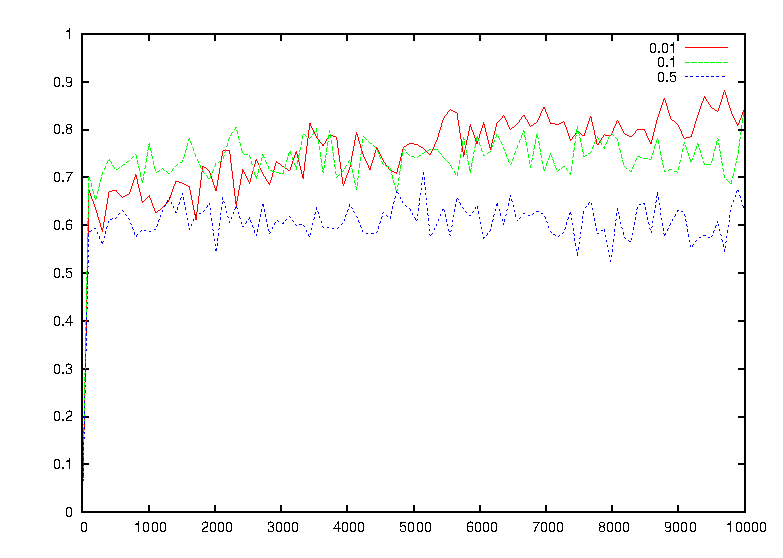
\includegraphics[width=0.9\textwidth]{figures/bandit_fixed_epsilon}
    \caption{$\epsilon_t = 0.1$, $\step \in \{0.01, 0.1, 0.5\}$.}
    \label{fig:bandit-fixed-epsilon}
  \end{figure}
\end{frame}

\begin{frame}
  \begin{figure}[H]
    \centering
    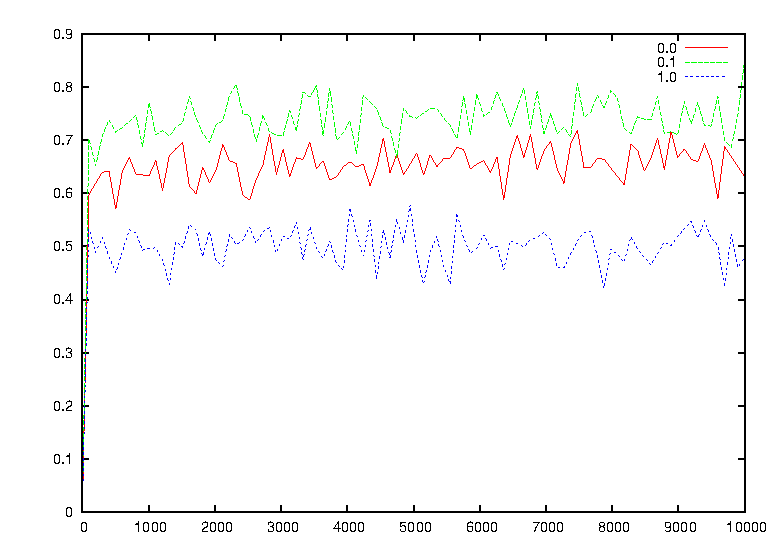
\includegraphics[width=0.9\textwidth]{figures/bandit_fixed_alpha}
    \caption{$\epsilon_t = \epsilon$, $\step = 0.1$.}
    \label{fig:bandit-fixed-alpha}
  \end{figure}
\end{frame}
\only<article>{
  The main two parameters of the algorithm are randomness $\epsilon$-greedy action selection and the step-size. Figures~\ref{fig:bandit-fixed-epsilon} and~\ref{fig:bandit-fixed-alpha} show the average reward obtained, if we keep the step size $\alpha$ or the randomness $\epsilon$ fixed, respectively. 
  We see that there the choice of values really affects convergence.

  For a fixed $\epsilon$, we find that larger values of $\alpha$ tend to give a better result eventually, while smaller values have a better initial performance. This is a natural trade-off, since large $\alpha$ appears to ``learn'' fast, but it also ``forgets'' quickly. That is, for a large $\alpha$, our estimates mostly depend upon the last few rewards observed.

  Things are not so clear-cut for the choice of $\epsilon$. We see that the choice of $\epsilon = 0$, is significantly worse than $\epsilon = 0.1$. So, that appears to suggest that there is an optimal level of exploration. How should that be determined? Ideally, we should be able to to use the decision-theoretic solution seen earlier, but perhaps a good heuristic way of choosing $\epsilon$ may be good enough.
}
\only<presentation>{
  \begin{frame}
    \begin{block}{Main idea of the algorithm}
      \begin{itemize}
      \item Estimate parameters
      \item Act according to the estimates
      \end{itemize}
    \end{block}

    \begin{block}{Requirements}
      \begin{itemize}
      \item Good estimation procedure.
      \item Balance estimation with getting rewards!
      \end{itemize}
    \end{block}
  \end{frame}
}

\subsection{Decision-theoretic bandit process}
\label{sec:decision-theoretic-bandits}

The basic bandit process can be seen in Figure~\ref{fig:basic-bandit-process}. We can now define the general decision-theoretic bandit process, not restricted to independent Bernoulli bandits.
\begin{definition}
  Let $\CA$ be a set of actions, not necessarily finite. Let $\Omega$ be a set of possible parameter values, indexing a family of probability measures $\family = \cset{P_{\omega, a}}{\omega \in \Omega, a \in \CA}$. There is some $\omega \in \Omega$ such that, whenever we take action $a_t = a$, we observe reward $r_t \in \CR \subset \Reals$ with probability measure:
  \begin{equation}
    \label{eq:bandit-reward-probability}
    P_{\omega,a}(R) \defn \Pr_\omega(r_{t} \in R \mid a_t = a),
    \qquad R \subseteq \Reals.
  \end{equation}
  Let $\bel_1$ be a prior distribution on $\Omega$ and let the posterior distributions be defined as:
  \begin{equation}
    \label{eq:bandit-posteriors}
    \bel_{t+1}(B) \propto \int_B P_{\omega, a_t} (r_t) \dd \bel_t(\omega).
  \end{equation}
  The next belief is random, since it depends on the random quantity $r_t$. In fact, the probability of the next reward lying in $R$ if $a_t = a$ is given by the following marginal distribution:
  \begin{equation}
    \label{eq:dt-bandit-reward-probability}
    P_{\bel_t, a} (R) \defn \int_\Omega P_{\omega,a}(R) \dd{\bel_t}(\omega).
  \end{equation}
  \begin{figure}[ht]
  \begin{center}
    \begin{tikzpicture}
      \node[RV] at (2,-1.5) (xn1) {$\bel_{t+1}^0$}; 
      \node[RV] at (2,-0.5) (xn2) {$\bel_{t+1}^1$};
      \node[RV] at (2,0.5) (xn3) {$\bel_{t+1}^2$}; 
      \node[RV] at (2,1.5) (xn4) {$\bel_{t+1}^3$};
      \node[select] at (0,-1) (an1) {$a^1_t$};
      \node[select] at (0,1) (an2) {$a^2_t$};
      \node[RV] at (-2,0) (xp) {$\bel_n$};
      \draw[->] (xp) -- (an1);
      \draw[->] (xp) -- (an2);
      \draw[->] (an1) -- (xn1) node[near start, below] {$r=0$};
      \draw[->] (an1) -- (xn2) node[near start, above] {$r=1$}; 
      \draw[->] (an2) -- (xn3) node[near start, below] {$r=0$}; 
      \draw[->] (an2) -- (xn4) node[near start, above] {$r=1$}; 
    \end{tikzpicture}
  \end{center}
  \caption{A partial view of the multi-stage process. Here, the probability that we obtain $r=1$ if we take action $a_t = i$ is simply $P_{\bel_t,i}(\{1\})$.}
  \label{fig:multi-stage-bandit}
\end{figure}  

  Finally, as $\bel_{t+1}$ deterministically depends on $\bel_t, a_t, r_t$, the probability of obtaining a particular next belief is the same as the probability of obtaining the corresponding rewards leading to the next belief. In more detail, we can write:
  \begin{equation}
    \label{eq:dt-bandit-belief-probability}
    \Pr(\bel_{t+1} = \bel \mid \bel_t, a_t)
    =
    \int_\CR \ind{\bel_{t}(\cdot \mid a_t, r_t = r) = \bel} \dd{P_{\bel_t, a}}(r). 
  \end{equation}
\end{definition}
In practice, although multiple reward sequences may lead to the same beliefs, we frequently ignore that possibility for simplicity. Then the process becomes a tree. A solution to the problem of what action to select is given by a backwards induction algorithm similar to that given in Section~\ref{sec:finite-horiz-backw}
\begin{block}{The backwards induction algorithm}
\begin{equation}
  U^*(\bel_t) = \max_{a_t} \E(r_t \mid \bel_t, a_t) + \sum_{\bel_{t+1}} \Pr(\bel_{t+1} \mid \bel_t, a_t) U^*(\bel_{t+1}).\label{eq:backwards-induction-bandits}
\end{equation}
\end{block}
The above equation is the \emindex{backwards induction} algorithm for bandits.  If you look at this structure, you can see that  next belief only depends on the current belief, action and reward, i.e. it satisfies the Markov property, as seen in Figure~\ref{fig:multi-stage-bandit}. Consequently, a decision-theoretic bandit process can be modelled more generally as a \index{Markov decision process}Markov decision process, explained in the following section. It turns out that backwards induction, as well as other efficient algorithms, can provide optimal solutions for Markov decision processes.
\begin{figure}[htb]
  \centering
  \begin{subfigure}{0.3\textwidth}
    \begin{tikzpicture}
      \node[select] at (0,1) (at) {$a_t$};
      \node[RV,hidden] at (0,-2) (omega) {$\omega$};
      \node[utility] at (1,-1) (rt) {$r_{t}$};
      \draw[->] (at) -- (rt);
      \draw[->] (omega) -- (rt);
      \node[select] at (0,1) (at2) {$a_{t+1}$};
      \node[utility] at (1,-1) (rt2) {$r_{t+1}$};
      \draw[->] (at2) -- (rt2);
      \draw[->] (omega) -- (rt2);
    \end{tikzpicture}
    \label{fig:basic-bandit-process}
  \end{subfigure}
  ~
  \begin{subfigure}{0.3\textwidth}
    \begin{tikzpicture}
      \node[RV,hidden] at (0,-2) (omega) {$\omega$};
      \node[RV] at (0,0) (bt) {$\bel_t$};
      \node[select] at (0,1) (at) {$a_t$};
      \node[utility] at (1,-1) (rt) {$r_{t}$};
      \draw[->] (omega) -- (rt);
      \draw[->] (at) -- (rt);
      \node[RV] at (2,0) (bt2) {$\bel_{t+1}$};
      \draw[->] (at) -- (bt2);
      \draw[->] (bt) -- (bt2);
      \draw[->] (rt) -- (bt2);
      \node[select] at (2,1) (at2) {$a_{t+1}$};
      \node[utility] at (3,-1) (rt2) {$r_{t+1}$};
      \draw[->] (omega) -- (rt2);
      \draw[->] (at2) -- (rt2);
    \end{tikzpicture}
    \label{fig:dt-bandit-full}
  \end{subfigure}
  \begin{subfigure}{0.3\textwidth}
      \begin{tikzpicture}
      \node[RV] at (0,0) (bt) {$\bel_t$};
      \node[select] at (0,1) (at) {$a_t$};
      \node[utility] at (1,-1) (rt) {$r_{t}$};
      \draw[->] (bt) -- (rt);
      \draw[->] (at) -- (rt);
      \node[RV] at (2,0) (bt2) {$\bel_{t+1}$};
      \draw[->] (at) -- (bt2);
      \draw[->] (bt) -- (bt2);
      \draw[->] (rt) -- (bt2);
      \node[select] at (2,1) (at2) {$a_{t+1}$};
      \node[utility] at (3,-1) (rt2) {$r_{t+1}$};
      \draw[->] (bt2) -- (rt2);
      \draw[->] (at2) -- (rt2);
    \end{tikzpicture}
    \label{fig:dt-bandit-lifted}
  \end{subfigure}
  \caption{Three views of the bandit process.
    Figure~\ref{fig:basic-bandit-process} shows the basic bandit
    process, from the view of an external observer. The decision maker
    selects $a_t$, while the parameter $\omega$ of the process is
    hidden. It then obtains reward $r_t$. The process repeats for $t =
    1, \ldots, T$.  The decision-theoretic bandit process is shown in
    Figures~\ref{fig:dt-bandit-full} and
    \ref{fig:dt-bandit-lifted}. While $\omega$ is not known, at each
    time step $t$ we maintain a belief $\bel_t$ on $\Omega$. The
    reward distribution is then defined through our belief. In
    Figure~\ref{fig:dt-bandit-full}, we can see that complete process,
    where the dependency on $\omega$ is clear. In
    Figure~\ref{fig:dt-bandit-lifted}, we marginalise out $\omega$ and
    obtain a model where the transitions only depend on the current
    belief and action.}
  \label{fig:bandit-process}
\end{figure}

In reality, the reward depends only on the action and the unknown $\omega$, as can be seen in Figure~\ref{fig:dt-bandit-full}. This is the point of view of an external observer. However, from the point of view of the decision maker, the distribution of $\omega$ only depends on his current belief. Consequently, the distribution of rewards also only depends on the current belief, as we can marginalise over $\omega$. This gives rise to the decision-theoretic bandit process shown in Figure~\ref{fig:dt-bandit-lifted}.
In the following section, we shall consider Markov decision processes more generally.


\section{Contextual Bandits}

\only<article>{
In the simplest bandit setting, our only information when selecting an arm is the sequence of previous plays and rewards obtained. However, in many cases we have 
\section{Experiment design}


%%% Local Variables:
%%% mode: latex
%%% TeX-master: "notes"
%%% End:
